\documentclass[main.tex]{subfiles}
\newcommand{\DiagramaEscala}{0.9}
\begin{document}

\section{Ajuste de curvas}

%--------------------------------------------------
% Diapositiva 1
%--------------------------------------------------
\subsection{Introducción}
% Introducción al problema
\begin{frame}{Estimaciones con datos discretos}
\begin{itemize}
  \item Los datos a menudo se presentan como valores \textbf{discretos} a lo largo de un continuo.
  \item Es necesario estimar valores en puntos intermedios \textbf{(interpolación)} o ajustar una función \textbf{simplificada} \textbf{(regresión)}.
  \item Estas estrategias se conocen como \textbf{ajuste de curvas}.
\end{itemize}
\end{frame}

% Métodos generales de ajuste
\begin{frame}{Métodos generales de ajuste de curvas}
\begin{block}{1. Regresión por mínimos cuadrados}
\begin{itemize}
  \item Se usa cuando los datos tienen \textbf{error o ruido}.
  \item La curva \textbf{no pasa por todos los puntos}, sino que representa la tendencia general.
  \item Método común: \textbf{mínimos cuadrados}.
\end{itemize}
\end{block}

\begin{block}{2. Interpolación}
\begin{itemize}
  \item Se usa con \textbf{datos precisos}, típicos de tablas.
  \item La curva \textbf{pasa exactamente por todos los puntos}.
  \item Ejemplos: tablas de densidad del agua, calor específico.
\end{itemize}
\end{block}
\end{frame}


% Antecedentes matemáticos
\begin{frame}{Antecedentes matemáticos}
\begin{itemize}
  \item Interpolación: basada en \textbf{series de Taylor} y \textbf{diferencias finitas divididas}.
  \item Regresión: requiere fundamentos de \textbf{estadística descriptiva}.
  \item Si conoce: media, desviación estándar, residuales, normalidad e intervalos, puede avanzar a la sección siguiente.
\end{itemize}
\end{frame}

% Estadística descriptiva
\begin{frame}{Estadística simple}
\begin{itemize}
  \item Se utilizan \textbf{estadísticos} para describir el centro y la dispersión de un conjunto de datos.
  \item \textbf{Media aritmética:} $\bar{y} = \frac{\sum y_i}{n}$
  \item \textbf{Desviación estándar:} $s_y = \sqrt{\frac{\sum (y_i - \bar{y})^2}{n-1}}   = \sqrt{\frac{S_t}{n-1}}  \Rightarrow s_t=\sum(y_i-\bar{y})^2$
  \item \textbf{Varianza:} $s_y^2  = \frac{\sum (y_i - \bar{y})^2}{n-1} \Rightarrow  s_y^2  = \frac{(\sum y_i^2 - (\sum{y_i})^2)/n}{n-1} $ 
  \item \textbf{Coeficiente de variación:} $\text{c.v.} = \frac{s_y}{\bar{y}} \times 100\%$
\end{itemize}
\end{frame}


% Cierre o resumen
\begin{frame}{Resumen}
\begin{itemize}
  \item El ajuste de curvas permite obtener valores intermedios o simplificar funciones complejas.
  \item Se escoge \textbf{regresión} si los datos son ruidosos, o \textbf{interpolación} si los datos son exactos.
  \item Estadísticos como la media y la desviación estándar ayudan a analizar la confiabilidad de los datos.
\end{itemize}
\end{frame}

\subsection{Regresión por mínimos cuadrados}

% Regresión con datos ruidosos
\begin{frame}{Ajuste con datos ruidosos: limitaciones de la interpolación}
\begin{itemize}
  \item Cuando hay \textbf{errores sustanciales}, la interpolación polinomial puede producir \textbf{oscilaciones indeseadas}.
  \item Un polinomio de alto grado puede pasar por todos los puntos, pero \textbf{exagerar la variabilidad}.
  \item Una mejor estrategia: \textbf{aproximar la tendencia general} sin forzar el paso por cada punto.
  \item Esto se logra mediante \textbf{regresión por mínimos cuadrados}, minimizando la discrepancia entre datos y curva.
\end{itemize}
\end{frame}

% --- Definición inicial ---
\begin{frame}{Introducción a la Regresión Lineal}
  \begin{itemize}
    \item Objetivo: Ajustar una línea recta a un conjunto de puntos \((x_i, y_i)\).
    \item Modelo matemático: \( y = a_0 + a_1x + e \)
    \item Donde:
    \begin{itemize}
      \item \(a_0\): Intersección con el eje y.
      \item \(a_1\): Pendiente.
      \item \(e\): Error o residuo \(e = y - a_0 - a_1x\)
    \end{itemize}
  \end{itemize}
\end{frame}

% --- Criterios para mejor ajuste ---
\begin{frame}{Criterios para un Mejor Ajuste}
  \begin{enumerate}
    \item Minimizar \( \sum e_i = \sum (y_i - a_0 - a_1x_i) \)
    \item Minimizar \[\sum_{i=1}^{n}  |e_i| = \sum_{i=1}^{n} |y_i - a_0 - a_1x_i| \]
    \item Criterio Minimax: Minimizar el error máximo.
    \item \textbf{Mejor criterio}: Minimizar la suma de los cuadrados de los residuos:
    \[
      S_r =\sum_{i=1}^{n}  |e_i| =\sum_{i=1}^n (y_{i,medida}-y_{i,modelo})^2 =\sum_{i=1}^n (y_i - a_0 - a_1x_i)^2
    \]
  \end{enumerate}
\end{frame}

% --- Derivación de mínimos cuadrados ---
\begin{frame}{Derivación del Método de Mínimos Cuadrados}
  \begin{itemize}
    \item Derivar \(S_r\) respecto a \(a_0\) y \(a_1\):
    \begin{align*}
      \frac{\partial S_r}{\partial a_0} &= -2 \sum (y_i - a_0 - a_1x_i) \\
      \frac{\partial S_r}{\partial a_1} &= -2 \sum x_i(y_i - a_0 - a_1x_i)
    \end{align*}
    \item Igualar a cero para minimizar:
    \begin{align*}
      \sum y_i &= na_0 + a_1 \sum x_i \\
      \sum x_iy_i &= a_0 \sum x_i + a_1 \sum x_i^2
    \end{align*}
  \end{itemize}
\end{frame}

% --- Ecuaciones normales ---
\begin{frame}{Sistema de Ecuaciones Normales}
  \begin{block}{Ecuaciones simultáneas}
    \begin{align*}
      na_0 + a_1 \sum x_i &= \sum y_i \\
      a_0 \sum x_i + a_1 \sum x_i^2 &= \sum x_iy_i
    \end{align*}
  \end{block}
  \begin{itemize}
    \item Se resuelven para obtener \(a_0\) y \(a_1\)
  \end{itemize}
\end{frame}

% --- Solución explícita ---
\begin{frame}{Solución Explícita de los Coeficientes}
  \begin{itemize}
    \item Pendiente \(a_1\):
    \[
      a_1 = \frac{n \sum x_iy_i - \sum x_i \sum y_i}{n \sum x_i^2 - (\sum x_i)^2}
    \]
    \item Intersección \(a_0\):
    \[
      a_0 = \bar{y} - a_1 \bar{x}
    \]
    \item Donde \(\bar{x}\) y \(\bar{y}\) son las medias de los datos.
  \end{itemize}
\end{frame}

% --- Ejemplo 17.1 ---
\begin{frame}{Ejemplo 1: Planteamiento del Problema}
  \begin{itemize}
    \item Ajustar una recta a los datos de la tabla:
  \end{itemize}
  \begin{center}
  \begin{tabular}{|c|c|}
    \hline
    $x_i$ & $y_i$ \\
    \hline
    1 & 0.5 \\
    2 & 2.5 \\
    3 & 2.0 \\
    4 & 4.0 \\
    5 & 3.5 \\
    6 & 6.0 \\
    7 & 5.5 \\
    \hline
  \end{tabular}
  \end{center}
\end{frame}

\begin{frame}{Cálculos y Resultados}
  \begin{itemize}
    \item Sumas:
    \begin{align*}
      n &= 7, & \sum x_i &= 28, & \sum y_i &= 24 \\
      \sum x_i^2 &= 140, & \sum x_iy_i &= 119.5 \\
      \bar{x} &= 4, & \bar{y} &= 3.428571
    \end{align*}
    \item Cálculo de los coeficientes:
    \begin{align*}
      a_1 &= \frac{7(119.5) - 28(24)}{7(140) - (28)^2} = 0.8392857 \\
      a_0 &= 3.428571 - 0.8392857(4) = 0.07142857
    \end{align*}
  \end{itemize}
\end{frame}

\begin{frame}{Ecuación de la Recta Ajustada}
  \begin{block}{Resultado final}
    \[
      y = 0.07142857 + 0.8392857x
    \]
  \end{block}
  \begin{itemize}
    \item Esta es la línea de mejor ajuste por mínimos cuadrados.
    \item Puede graficarse junto con los puntos originales.
  \end{itemize}
\end{frame}
\begin{frame}{Gráfica del Ajuste}
  \begin{center}
    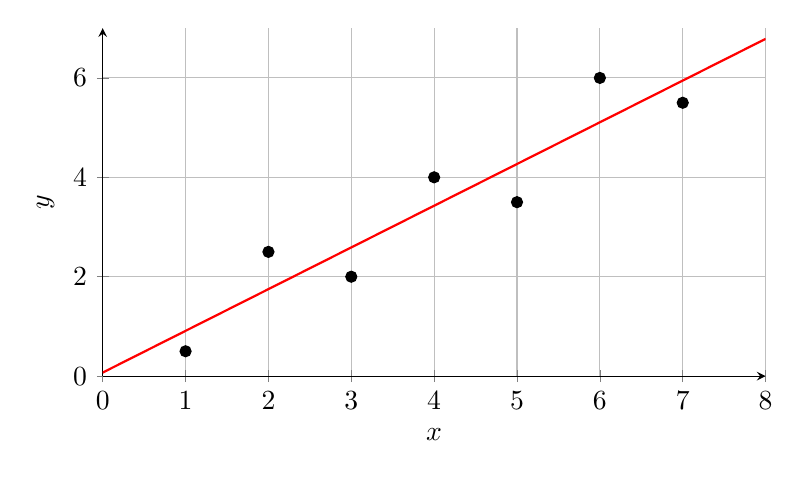
\begin{tikzpicture}
      \begin{axis}[
        axis lines = left,
        xlabel = $x$,
        ylabel = $y$,
        xmin=0, xmax=8,
        ymin=0, ymax=7,
        grid=both,
        width=10cm, height=6cm
      ]
      \addplot[only marks, mark=*] coordinates {
        (1,0.5) (2,2.5) (3,2.0) (4,4.0) (5,3.5) (6,6.0) (7,5.5)
      };
      \addplot[domain=0:8, samples=100, thick, red] {0.07142857 + 0.8392857*x};
      \end{axis}
    \end{tikzpicture}
  \end{center}
\end{frame}

\begin{frame}{Error en la Regresión Lineal}
  \begin{itemize}
    \item La línea obtenida por mínimos cuadrados es única.
    \item Minimiza la suma de los cuadrados de los residuos:
    \[
      S_r =\sum_{i=1}^n (e_i)^2 = \sum_{i=1}^n (y_i - a_0 - a_1x_i)^2
    \]
    \item Cualquier otra línea genera mayor error.
  \end{itemize}
\end{frame}

\begin{frame}{Analogía con la Media}
  \begin{itemize}
    \item El ajuste lineal minimiza la distancia vertical entre los puntos y la línea.
    \item Similar a cómo la media minimiza la suma de las desviaciones cuadradas respecto a \(\bar{y}\).
    \item La línea se interpreta como una tendencia central generalizada.
  \end{itemize}
\end{frame}

\begin{frame}{Principio de Máxima Verosimilitud}
  \begin{itemize}
    \item Si se cumplen dos condiciones:
    \begin{enumerate}
      \item Varianza constante en todo el rango de datos.
      \item Distribución normal de los errores.
    \end{enumerate}
    \item Entonces, el modelo lineal es óptimo según el criterio de máxima verosimilitud.
    \item Fuente: Draper y Smith (1981).
  \end{itemize}
\end{frame}

\begin{frame}{Error Estándar de la Estimación}
  \begin{itemize}
    \item Mide la dispersión de los datos respecto a la línea:
    \[
      s_{y/x} = \sqrt{\frac{S_r}{n - 2}}
    \]
    \item Se divide entre \(n - 2\) porque se estimaron dos parámetros: \(a_0\) y \(a_1\).
    \item Similar al cálculo de la desviación estándar con pérdida de grados de libertad.
  \end{itemize}
  \begin{itemize}
    \item \(s_y\): dispersión de los datos respecto a la media.
    \item \(s_{y/x}\): dispersión de los datos respecto a la línea de regresión.
    \item Permite evaluar la precisión del modelo lineal.
  \end{itemize}
\end{frame}

\begin{frame}{Coeficiente de Determinación \(r^2\)}
  \begin{itemize}
    \item Mide la proporción de la variabilidad explicada por el modelo.
    \item Definido como:
    \[
      r^2 = \frac{S_t - S_r}{S_t}
    \]
    \item Donde:
    \begin{itemize}
      \item \(S_t\): suma total de cuadrados respecto a \(\bar{y}\).
      \item \(S_r\): suma de los residuos cuadráticos.
    \end{itemize}
    \item Valores:
    \begin{itemize}
      \item \(r^2 = 1\): ajuste perfecto.
      \item \(r^2 = 0\): la recta no mejora respecto a la media.
    \end{itemize}
  \end{itemize}
\end{frame}

\begin{frame}{Fórmula alternativa de \(r\)}
  \begin{itemize}
    \item El coeficiente de correlación también puede calcularse como:
    \[
    r = \frac{n\sum x_i y_i - \sum x_i \sum y_i}
             {\sqrt{n \sum x_i^2 - (\sum x_i)^2} \sqrt{n \sum y_i^2 - (\sum y_i)^2}}
    \]
    \item Esta expresión es más adecuada para programación computacional.
    \item \(r^2\) se obtiene simplemente elevando \(r\) al cuadrado.
  \end{itemize}
\end{frame}

\begin{frame}{Ejemplo 2 – Estimación de Errores}
  \textbf{Datos base:} ejemplo 1 con \( n = 7 \)
  \begin{itemize}
    \item \(\sum (y_i - \bar{y})^2 = S_t = 22.7143\)
    \item \(\sum (y_i - a_0 - a_1x_i)^2 = S_r = 2.9911\)
  \end{itemize}
  \textbf{Cálculos:}
  \begin{itemize}
    \item Desviación estándar total:
    \[
      s_y = \sqrt{\frac{22.7143}{6}} = 1.9457
    \]
    \item Error estándar del estimado:
    \[
      s_{y/x} = \sqrt{\frac{2.9911}{5}} = 0.7735
    \]
  \end{itemize}
\end{frame}

\begin{frame}{Interpretación del Ajuste}
  \begin{itemize}
    \item Como \( s_{y/x} < s_y \), el ajuste es adecuado.
    \item Coeficiente de determinación:
    \[
      r^2 = \frac{22.7143 - 2.9911}{22.7143} = 0.868
    \]
    \item Coeficiente de correlación:
    \[
      r = \sqrt{0.868} = 0.932
    \]
    \item El modelo explicó el 86.8\% de la variabilidad.
  \end{itemize}
\end{frame}

\subsection{Linealización de Relaciones No Lineales}
\begin{frame}{Linealización de Relaciones No Lineales}
  \begin{itemize}
    \item La regresión lineal requiere una relación lineal entre variables.
    \item Muchas relaciones en ingeniería son no lineales.
    \item Podemos aplicar transformaciones para linealizar modelos no lineales.
    \item Esto permite usar métodos de regresión lineal para ajustarlos.
  \end{itemize}
\end{frame}

\begin{frame}{Modelo Exponencial}
  \[
    y = a_1 e^{b_1 x}
  \]
  \begin{itemize}
    \item Se linealiza aplicando logaritmo natural:
    \[
      \ln y = \ln a_1 + b_1 x
    \]
    \item Forma lineal: \( Y = A + Bx \) donde:
    \begin{itemize}
      \item \( Y = \ln y \)
      \item \( A = \ln a_1 \), \( B = b_1 \)
    \end{itemize}
    \item Gráfica de \( \ln y \) vs. \( x \): línea recta
  \end{itemize}
\end{frame}

\begin{frame}{Modelo de Potencias}
  \[
    y = a_2 x^{b_2}
  \]
  \begin{itemize}
    \item Se linealiza aplicando logaritmo en base 10:
    \[
      \log y = b_2 \log x + \log a_2
    \]
    \item Forma lineal: \( Y = B X + A \) donde:
    \begin{itemize}
      \item \( Y = \log y \), \( X = \log x \)
      \item \( A = \log a_2 \), \( B = b_2 \)
    \end{itemize}
    \item Gráfica de \( \log y \) vs. \( \log x \): línea recta
  \end{itemize}
\end{frame}

\begin{frame}{Modelo de Razón de Crecimiento}
  \[
    y = \frac{a_3 x}{b_3 + x}
  \]
  \begin{itemize}
    \item Se linealiza tomando recíprocos:
    \[
      \frac{1}{y} = \frac{1}{a_3} + \frac{b_3}{a_3} \cdot \frac{1}{x}
    \]
    \item Forma lineal: \( Y = A + B X \) donde:
    \begin{itemize}
      \item \( Y = \frac{1}{y} \), \( X = \frac{1}{x} \)
      \item \( A = \frac{1}{a_3} \), \( B = \frac{b_3}{a_3} \)
    \end{itemize}
    \item Gráfica de \( 1/y \) vs. \( 1/x \): línea recta
  \end{itemize}
\end{frame}

\begin{frame}{Ventajas de la Linealización}
  \begin{itemize}
    \item Permite aplicar regresión lineal a modelos originalmente no lineales.
    \item Simplifica el cálculo de parámetros.
    \item Se puede volver a la forma original del modelo para interpretación y predicción.
    \item Aplicaciones frecuentes:
    \begin{itemize}
      \item Crecimiento poblacional
      \item Decaimiento radiactivo
      \item Transferencia de calor
    \end{itemize}
  \end{itemize}
\end{frame}

\begin{frame}{Resumen}
  \begin{itemize}
    \item Graficar los datos siempre es el primer paso.
    \item Si no hay relación lineal, evaluar posibles transformaciones.
    \item Aplicar la regresión lineal sobre los datos transformados.
    \item Revertir la transformación para interpretar el modelo original.
  \end{itemize}
\end{frame}

\begin{frame}{Planteamiento del Problema}
  \small
  Ajustar el modelo:
  \[
    y = a_2 x^{b_2}
  \]
  a los siguientes datos experimentales mediante transformación logarítmica:

  \begin{center}
    \begin{tabular}{cc|cc}
    \hline
    \(x\) & \(y\) & \(\log x\) & \(\log y\) \\
    \hline
    1 & 0.5 & 0.000 & -0.301 \\
    2 & 1.7 & 0.301 & 0.226 \\
    3 & 3.4 & 0.477 & 0.534 \\
    4 & 5.7 & 0.602 & 0.753 \\
    5 & 8.4 & 0.699 & 0.922 \\
    \hline
    \end{tabular}
  \end{center}
\end{frame}

\begin{frame}{Transformación y Regresión}
  \small
  Se aplica logaritmo decimal a ambos lados:
  \[
    \log y = \log a_2 + b_2 \log x
  \]
  \textbf{Regresión lineal:}
  \begin{itemize}
    \item Pendiente \(b_2 = 1.329\)
    \item Intersección \(\log a_2 = -0.300 \Rightarrow a_2 \approx 0.501\)
  \end{itemize}
  \textbf{Modelo ajustado:}
  \[
    y = 0.501 \, x^{1.329}
  \]
\end{frame}

\begin{frame}{Gráfica de los Datos Originales}
  \begin{center}
  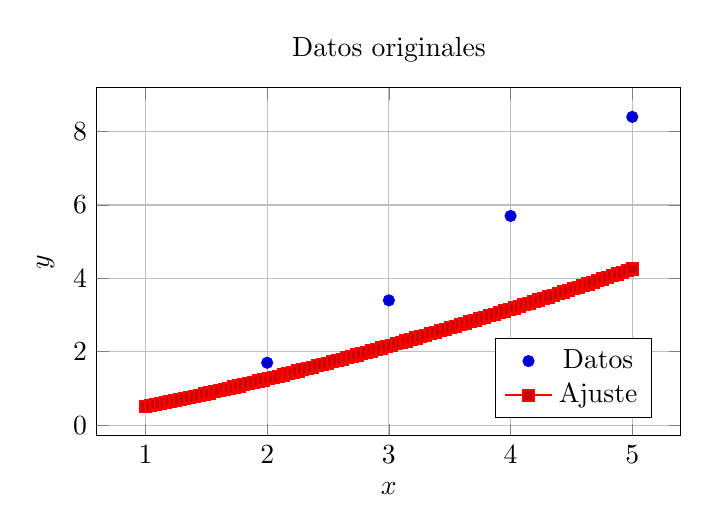
\begin{tikzpicture}
    \begin{axis}[
      width=9cm,
      height=6cm,
      xlabel={$x$},
      ylabel={$y$},
      grid=both,
      title={Datos originales},
      legend style={at={(0.95,0.05)}, anchor=south east}
    ]
    \addplot+[only marks, mark=*] coordinates {
      (1,0.5) (2,1.7) (3,3.4) (4,5.7) (5,8.4)
    };
    \addplot+[domain=1:5, samples=100, thick] {0.501*x^1.329};
    \legend{Datos, Ajuste}
    \end{axis}
  \end{tikzpicture}
  \end{center}
\end{frame}

\begin{frame}{Gráfica de los Datos Transformados (log-log)}
  \begin{center}
  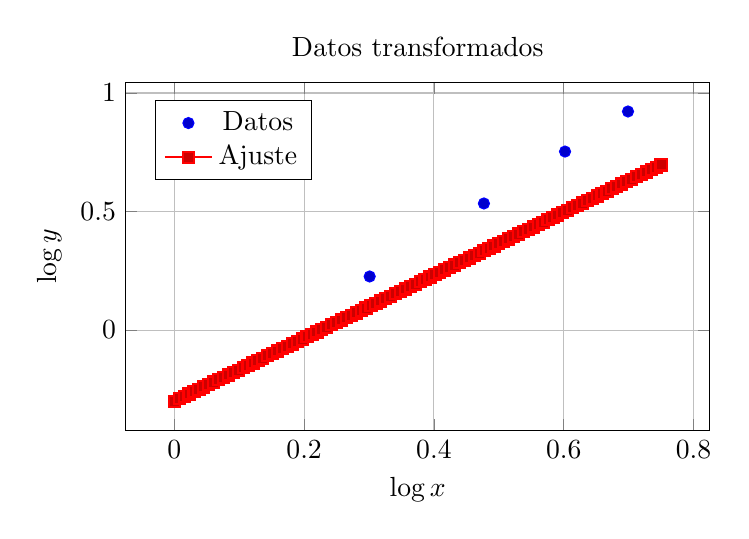
\begin{tikzpicture}
    \begin{axis}[
      width=9cm,
      height=6cm,
      xlabel={$\log x$},
      ylabel={$\log y$},
      grid=both,
      title={Datos transformados},
      legend style={at={(0.05,0.95)}, anchor=north west}
    ]
    \addplot+[only marks, mark=*] coordinates {
      (0.000, -0.301)
      (0.301, 0.226)
      (0.477, 0.534)
      (0.602, 0.753)
      (0.699, 0.922)
    };
    \addplot+[domain=0:0.75, samples=100, thick] {-0.300 + 1.329*x};
    \legend{Datos, Ajuste}
    \end{axis}
  \end{tikzpicture}
  \end{center}
\end{frame}

\begin{frame}{Comentarios Generales sobre la Regresión Lineal}
  \begin{itemize}
    \item La regresión lineal tiene supuestos estadísticos importantes:
    \begin{enumerate}
      \item Los valores de \(x\) son conocidos, fijos y sin error.
      \item Los valores de \(y\) son variables aleatorias independientes con igual varianza.
      \item Para un \(x\) dado, los \(y\) están normalmente distribuidos.
    \end{enumerate}
    \item Estos supuestos permiten una interpretación estadística rigurosa.
    \item La regresión de \(y\) contra \(x\) no es igual a la regresión de \(x\) contra \(y\).
  \end{itemize}
\end{frame}

\begin{frame}{Planteamiento del Problema}
  \small
  Ajustar el modelo exponencial:
  \[
    y = a_1 e^{b_1 x}
  \]
  a los siguientes datos experimentales mediante transformación logarítmica natural:

  \begin{center}
    \begin{tabular}{ccc}
    \hline
    \(x\) & \(y\) & \(\ln y\) \\
    \hline
    1 & 2.7 & 0.993 \\
    2 & 7.4 & 2.001 \\
    3 & 20.1 & 3.004 \\
    4 & 54.6 & 4.000 \\
    5 & 148.4 & 5.001 \\
    \hline
    \end{tabular}
  \end{center}
\end{frame}

\begin{frame}{Transformación y Regresión}
  \small
  Se aplica logaritmo natural a ambos lados:
  \[
    \ln y = \ln a_1 + b_1 x
  \]
  \textbf{Regresión lineal:}
  \begin{itemize}
    \item Pendiente \(b_1 = 1.001\)
    \item Intersección \(\ln a_1 = -0.010 \Rightarrow a_1 = e^{-0.010} \approx 0.990\)
  \end{itemize}
  \textbf{Modelo ajustado:}
  \[
    y = 0.990 \, e^{1.001x}
  \]
\end{frame}

\begin{frame}{Gráfica de los Datos Originales}
  \begin{center}
  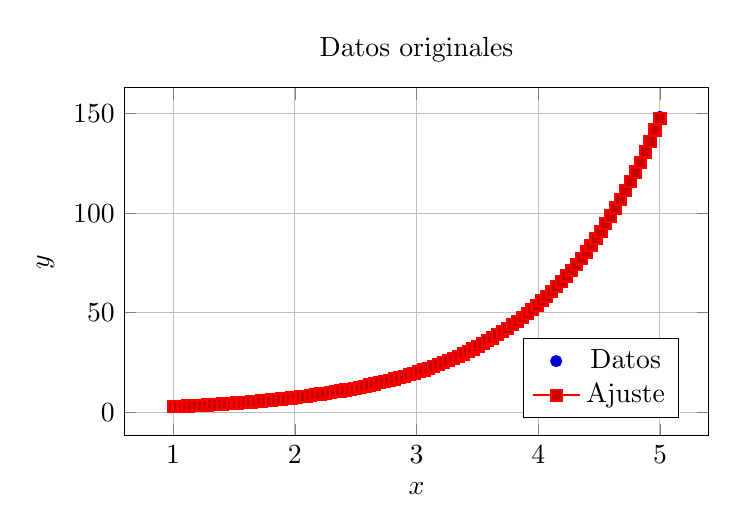
\begin{tikzpicture}
    \begin{axis}[
      width=9cm,
      height=6cm,
      xlabel={$x$},
      ylabel={$y$},
      grid=both,
      title={Datos originales},
      legend style={at={(0.95,0.05)}, anchor=south east}
    ]
    \addplot+[only marks, mark=*] coordinates {
      (1,2.7) (2,7.4) (3,20.1) (4,54.6) (5,148.4)
    };
    \addplot+[domain=1:5, samples=100, thick] {0.990*exp(1.001*x)};
    \legend{Datos, Ajuste}
    \end{axis}
  \end{tikzpicture}
  \end{center}
\end{frame}

\begin{frame}{Gráfica de los Datos Transformados (ln y vs. x)}
  \begin{center}
  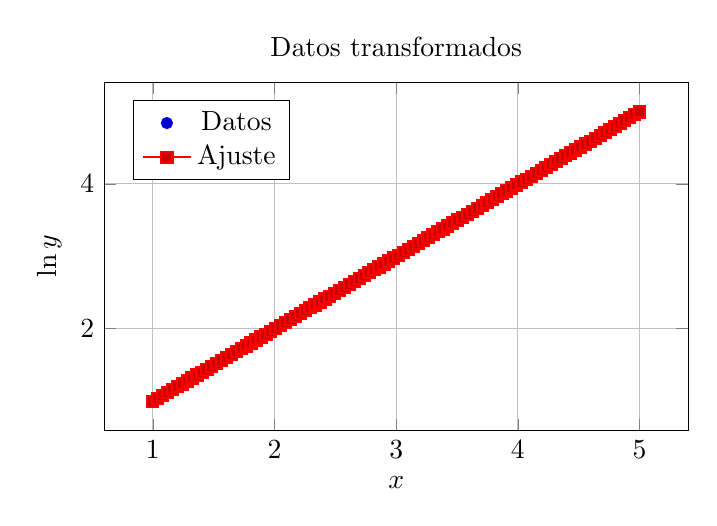
\begin{tikzpicture}
    \begin{axis}[
      width=9cm,
      height=6cm,
      xlabel={$x$},
      ylabel={$\ln y$},
      grid=both,
      title={Datos transformados},
      legend style={at={(0.05,0.95)}, anchor=north west}
    ]
    \addplot+[only marks, mark=*] coordinates {
      (1, 0.993)
      (2, 2.001)
      (3, 3.004)
      (4, 4.000)
      (5, 5.001)
    };
    \addplot+[domain=1:5, samples=100, thick] {-0.010 + 1.001*x};
    \legend{Datos, Ajuste}
    \end{axis}
  \end{tikzpicture}
  \end{center}
\end{frame}

\begin{frame}{Comentarios Finales}
  \begin{itemize}
    \item El modelo ajustado representa crecimiento exponencial:
    \[
      y = 0.990 \, e^{1.001x}
    \]
    \item La transformación logarítmica natural permitió aplicar regresión lineal.
    \item Se puede volver al modelo original para predicciones.
    \item Técnica útil para crecimiento poblacional, procesos químicos, economía, etc.
  \end{itemize}
\end{frame}
\begin{frame}{Planteamiento del Problema}
  \small
  Ajustar el modelo:
  \[
    y = \frac{a_3 x}{b_3 + x}
  \]
  a los siguientes datos experimentales, mediante transformación recíproca:

  \begin{center}
    \begin{tabular}{ccc|cc}
    \hline
    \(x\) & \(y\) &  & \(1/x\) & \(1/y\) \\
    \hline
    1 & 0.33 &  & 1.000 & 3.030 \\
    2 & 0.50 &  & 0.500 & 2.000 \\
    4 & 0.67 &  & 0.250 & 1.493 \\
    6 & 0.75 &  & 0.167 & 1.333 \\
    10 & 0.83 & & 0.100 & 1.205 \\
    \hline
    \end{tabular}
  \end{center}
\end{frame}

\begin{frame}{Transformación y Regresión}
  \small
  Transformación:
  \[
    \frac{1}{y} = \frac{1}{a_3} + \frac{b_3}{a_3} \cdot \frac{1}{x}
  \]
  \textbf{Regresión lineal sobre \(\frac{1}{y}\) vs. \(\frac{1}{x}\):}
  \begin{itemize}
    \item Pendiente \(B = \frac{b_3}{a_3} = 2.000\)
    \item Intersección \(A = \frac{1}{a_3} = 1.000 \Rightarrow a_3 = 1.000\)
    \item Entonces \(b_3 = 2.000\)
  \end{itemize}
  \textbf{Modelo ajustado:}
  \[
    y = \frac{1.0 \, x}{2.0 + x}
  \]
\end{frame}

\begin{frame}{Gráfica de los Datos Originales}
  \begin{center}
  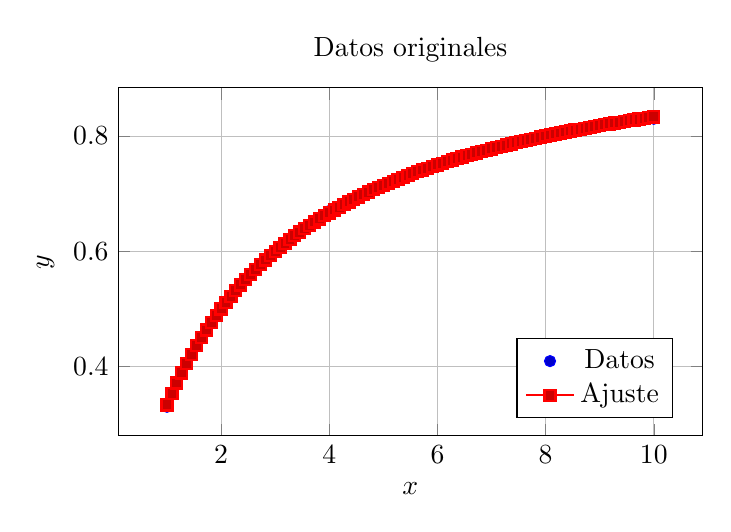
\begin{tikzpicture}
    \begin{axis}[
      width=9cm,
      height=6cm,
      xlabel={$x$},
      ylabel={$y$},
      grid=both,
      title={Datos originales},
      legend style={at={(0.95,0.05)}, anchor=south east}
    ]
    \addplot+[only marks, mark=*] coordinates {
      (1,0.33) (2,0.50) (4,0.67) (6,0.75) (10,0.83)
    };
    \addplot+[domain=1:10, samples=100, thick] {x/(2.0 + x)};
    \legend{Datos, Ajuste}
    \end{axis}
  \end{tikzpicture}
  \end{center}
\end{frame}

\begin{frame}{Gráfica Transformada (1/y vs. 1/x)}
  \begin{center}
  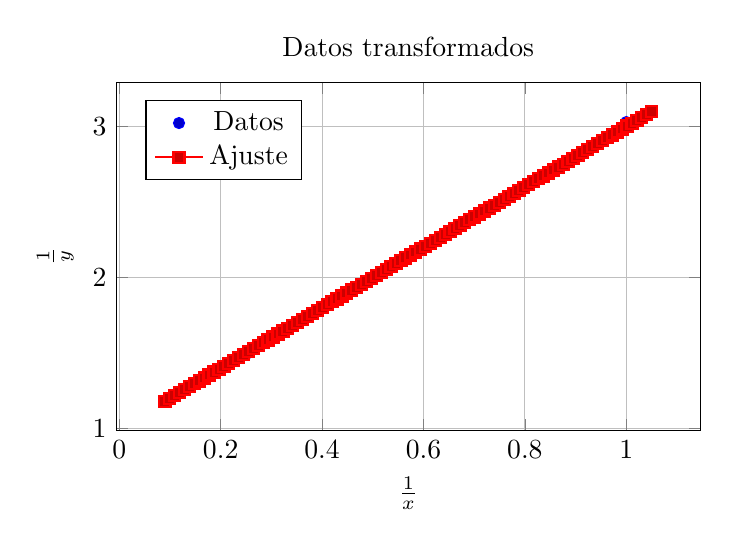
\begin{tikzpicture}
    \begin{axis}[
      width=9cm,
      height=6cm,
      xlabel={$\frac{1}{x}$},
      ylabel={$\frac{1}{y}$},
      grid=both,
      title={Datos transformados},
      legend style={at={(0.05,0.95)}, anchor=north west}
    ]
    \addplot+[only marks, mark=*] coordinates {
      (1.000, 3.030)
      (0.500, 2.000)
      (0.250, 1.493)
      (0.167, 1.333)
      (0.100, 1.205)
    };
    \addplot+[domain=0.09:1.05, samples=100, thick] {1.0 + 2.0*x};
    \legend{Datos, Ajuste}
    \end{axis}
  \end{tikzpicture}
  \end{center}
\end{frame}

\begin{frame}{Comentarios Finales}
  \begin{itemize}
    \item El modelo ajustado fue:
    \[
      y = \frac{1.0 \, x}{2.0 + x}
    \]
    \item Comportamiento típico de crecimiento limitado o saturado.
    \item La linealización recíproca facilita aplicar regresión lineal simple.
    \item Usado en:
    \begin{itemize}
      \item Cinética enzimática
      \item Ecología
      \item Procesos logísticos
    \end{itemize}
  \end{itemize}
\end{frame}

\subsection{regresión polinomial}
\begin{frame}{¿Por qué usar regresión polinomial?}
  \begin{itemize}
    \item Algunos datos presentan una tendencia curvilínea que no puede modelarse con una recta.
    \item Alternativa a las transformaciones no lineales: ajustar un polinomio directamente.
    \item Ampliación del modelo lineal para capturar comportamientos más complejos.
  \end{itemize}
\end{frame}

\begin{frame}{Modelo Polinomial de Segundo Grado}
  \[
    y = a_0 + a_1 x + a_2 x^2 + e
  \]
  \begin{itemize}
    \item El objetivo es minimizar la suma de los cuadrados de los residuos:
    \[
      S_r = \sum_{i=1}^{n} (y_i - a_0 - a_1 x_i - a_2 x_i^2)^2
    \]
    \item Se deriva con respecto a cada coeficiente \(a_0, a_1, a_2\) y se iguala a cero.
  \end{itemize}
\end{frame}

\begin{frame}{Ecuaciones Normales para Polinomio Cuadrático}
  \small
  \[
  \begin{aligned}
    n a_0 + \sum x_i a_1 + \sum x_i^2 a_2 &= \sum y_i \\
    \sum x_i a_0 + \sum x_i^2 a_1 + \sum x_i^3 a_2 &= \sum x_i y_i \\
    \sum x_i^2 a_0 + \sum x_i^3 a_1 + \sum x_i^4 a_2 &= \sum x_i^2 y_i
  \end{aligned}
  \]
  \begin{itemize}
    \item Es un sistema de 3 ecuaciones lineales con 3 incógnitas.
    \item Se resuelve usando métodos algebraicos o computacionales.
  \end{itemize}
\end{frame}

\begin{frame}{Modelo General de Grado \(m\)}
  \[
    y = a_0 + a_1 x + a_2 x^2 + \cdots + a_m x^m + e
  \]
  \begin{itemize}
    \item Extensión natural del modelo cuadrático.
    \item Requiere resolver un sistema de \(m + 1\) ecuaciones lineales.
    \item Cada coeficiente se asocia a un grado del polinomio.
  \end{itemize}
\end{frame}

\begin{frame}{Error Estándar en Regresión Polinomial}
  \[
    s_{y/x} = \sqrt{ \frac{S_r}{n - (m + 1)} }
  \]
  \begin{itemize}
    \item \(S_r\): suma de los cuadrados de los residuos.
    \item \(n\): número de datos.
    \item \(m + 1\): número de coeficientes ajustados.
    \item Cuantifica la dispersión de los datos alrededor del polinomio ajustado.
  \end{itemize}
\end{frame}

\begin{frame}{Coeficiente de Determinación \(r^2\)}
  \[
    r^2 = \frac{S_t - S_r}{S_t}
  \]
  \begin{itemize}
    \item Evalúa qué tan bien el modelo ajustado explica la variabilidad de los datos.
    \item Valores:
    \begin{itemize}
      \item \(r^2 = 1\): ajuste perfecto.
      \item \(r^2 = 0\): el modelo no mejora respecto a la media.
    \end{itemize}
    \item Se calcula igual que en regresión lineal simple.
  \end{itemize}
\end{frame}

\begin{frame}{Resumen}
  \begin{itemize}
    \item La regresión polinomial permite ajustar curvas de mayor complejidad.
    \item Se basa en el mismo criterio de mínimos cuadrados.
    \item Es útil cuando los datos muestran patrones curvos.
    \item Se deben evaluar tanto el error estándar como el \(r^2\) para validar el ajuste.
  \end{itemize}
\end{frame}

\begin{frame}{Ejemplo 5 – Regresión Polinomial Cuadrática}
  \textbf{Objetivo:} Ajustar los datos a un polinomio de segundo grado:
  \[
  y = a_0 + a_1 x + a_2 x^2
  \]
  \textbf{Datos:}
  \begin{tabular}{cc}
  \hline
  \(x_i\) & \(y_i\) \\
  \hline
  0 & 2.1 \\
  1 & 7.7 \\
  2 & 13.6 \\
  3 & 27.2 \\
  4 & 40.9 \\
  5 & 61.1 \\
  \hline
  \end{tabular}
\end{frame}

\begin{frame}{Ecuaciones Normales}
  \small
  A partir de los datos:
  \[
  \sum x = 15,\quad \sum x^2 = 55,\quad \sum x^3 = 225,\quad \sum x^4 = 979
  \]
  \[
  \sum y = 152.6,\quad \sum x y = 585.6,\quad \sum x^2 y = 2488.8
  \]

  El sistema de ecuaciones normales es:
  \[
  \begin{aligned}
  6 a_0 + 15 a_1 + 55 a_2 &= 152.6 \\
  15 a_0 + 55 a_1 + 225 a_2 &= 585.6 \\
  55 a_0 + 225 a_1 + 979 a_2 &= 2488.8
  \end{aligned}
  \]
\end{frame}

\begin{frame}{Solución y Modelo Ajustado}
  Resolviendo por eliminación de Gauss:
  \[
  \begin{aligned}
  a_0 &= 2.47857 \\
  a_1 &= 2.35929 \\
  a_2 &= 1.86071
  \end{aligned}
  \]

  El modelo cuadrático ajustado es:
  \[
  y = 2.47857 + 2.35929x + 1.86071x^2
  \]
\end{frame}

\begin{frame}{Evaluación del Ajuste}
  \small
  \textbf{Error estándar:}
  \[
  s_{y/x} = \sqrt{ \frac{3.74657}{6 - 3} } = 1.12
  \]

  \textbf{Coeficiente de determinación:}
  \[
  r^2 = \frac{2513.39 - 3.74657}{2513.39} = 0.99851
  \]
  \[
  r = \sqrt{0.99851} = 0.99925
  \]

  El modelo explica el 99.851\% de la variabilidad de los datos.
\end{frame}

\begin{frame}{Algoritmo para Regresión Polinomial}
  \begin{enumerate}
    \item Ingresar el grado del polinomio \(m\).
    \item Ingresar el número de datos \(n\).
    \item Si \(n < m + 1\), detener con error.
    \item Calcular la matriz aumentada con sumatorias.
    \item Resolver el sistema con eliminación de Gauss.
    \item Imprimir coeficientes \(a_0, a_1, ..., a_m\).
  \end{enumerate}
\end{frame}

\begin{frame}{Comentarios Finales}
  \begin{itemize}
    \item La regresión polinomial ajusta muy bien si se elige el grado adecuado.
    \item Para el ejemplo, el ajuste cuadrático fue excelente con \(r^2 \approx 0.999\).
    \item El algoritmo es fácilmente programable en cualquier lenguaje.
    \item Validar siempre con error estándar y coeficiente de determinación.
  \end{itemize}
\end{frame}
\begin{frame}{Gráfica del Ajuste Polinomial}
  \begin{center}
  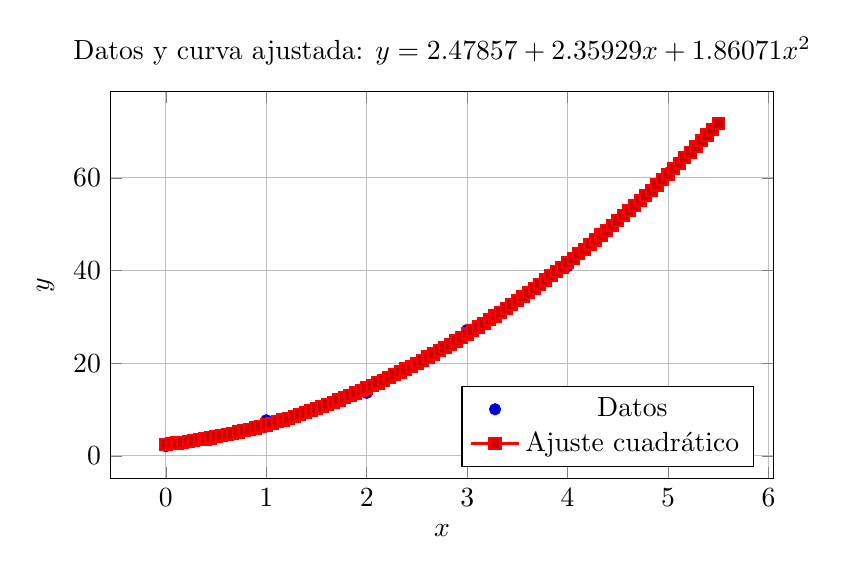
\begin{tikzpicture}
    \begin{axis}[
      width=10cm,
      height=6.5cm,
      xlabel={$x$},
      ylabel={$y$},
      grid=both,
      title={Datos y curva ajustada: $y = 2.47857 + 2.35929x + 1.86071x^2$},
      legend style={at={(0.97,0.03)}, anchor=south east},
      domain=0:5.5,
      samples=100
    ]
    % Datos originales
    \addplot+[only marks, mark=*] coordinates {
      (0,2.1) (1,7.7) (2,13.6) (3,27.2) (4,40.9) (5,61.1)
    };
    % Curva ajustada
    \addplot+[thick] {2.47857 + 2.35929*x + 1.86071*x^2};
    \legend{Datos, Ajuste cuadrático}
    \end{axis}
  \end{tikzpicture}
  \end{center}
\end{frame}


\begin{frame}{Introducción a la Regresión Múltiple}
  \begin{itemize}
    \item Extiende la regresión lineal simple a más de una variable independiente.
    \item Modelo general:
    \[
      y = a_0 + a_1 x_1 + a_2 x_2 + \dots + a_m x_m + e
    \]
    \item En el caso de dos variables, el modelo representa un plano en 3D.
  \end{itemize}
\end{frame}

\begin{frame}{Suma de Cuadrados de los Residuos}
  \[
    S_r = \sum_{i=1}^{n} (y_i - a_0 - a_1 x_{1i} - a_2 x_{2i})^2
  \]
  \begin{itemize}
    \item Derivando respecto a cada coeficiente se obtienen ecuaciones normales.
    \item El sistema puede expresarse en forma matricial y resolverse por eliminación de Gauss.
  \end{itemize}
\end{frame}
\begin{frame}{Derivación de las Ecuaciones Normales}
  \small
  Se parte del modelo:
  \[
    y = a_0 + a_1 x_1 + a_2 x_2 + e
  \]
  La suma de los cuadrados de los residuos es:
  \[
    S_r = \sum_{i=1}^n \left( y_i - a_0 - a_1 x_{1,i} - a_2 x_{2,i} \right)^2
  \]

  Derivando respecto a los coeficientes:
  \[
  \begin{aligned}
    \frac{\partial S_r}{\partial a_0} &= -2 \sum (y_i - a_0 - a_1 x_{1,i} - a_2 x_{2,i}) \\
    \frac{\partial S_r}{\partial a_1} &= -2 \sum x_{1,i}(y_i - a_0 - a_1 x_{1,i} - a_2 x_{2,i}) \\
    \frac{\partial S_r}{\partial a_2} &= -2 \sum x_{2,i}(y_i - a_0 - a_1 x_{1,i} - a_2 x_{2,i})
  \end{aligned}
  \]

  Igualando a cero, se obtienen las ecuaciones normales.
\end{frame}

\begin{frame}{Ecuaciones Normales en Forma Matricial}
  \small
  Las derivadas igualadas a cero generan el siguiente sistema:

  \[
  \begin{bmatrix}
    n & \sum x_1 & \sum x_2 \\
    \sum x_1 & \sum x_1^2 & \sum x_1 x_2 \\
    \sum x_2 & \sum x_1 x_2 & \sum x_2^2 \\
  \end{bmatrix}
  \begin{bmatrix}
    a_0 \\ a_1 \\ a_2
  \end{bmatrix}
  =
  \begin{bmatrix}
    \sum y \\ \sum x_1 y \\ \sum x_2 y
  \end{bmatrix}
  \]

  \vspace{1em}
  Esta forma es generalizable para regresión múltiple con \(m\) variables.
\end{frame}

\begin{frame}{Ejemplo 17.6 – Datos de Entrada}
  \small
  \textbf{Modelo:} \( y = a_0 + a_1 x_1 + a_2 x_2 \)

  \textbf{Datos:}
  \begin{tabular}{ccc}
    \hline
    \(x_1\) & \(x_2\) & \(y\) \\
    \hline
    0 & 0 & 5 \\
    2 & 1 & 10 \\
    2.5 & 2 & 9 \\
    1 & 3 & 0 \\
    4 & 6 & 3 \\
    7 & 2 & 27 \\
    \hline
  \end{tabular}
\end{frame}

\begin{frame}{Ejemplo 17.6 – Cálculo de Sumatorias}
  \small
  \[
    \begin{aligned}
      \sum y &= 54,\quad \sum x_1 = 16.5,\quad \sum x_2 = 14 \\
      \sum x_1^2 &= 76.25,\quad \sum x_2^2 = 54,\quad \sum x_1 x_2 = 48 \\
      \sum x_1 y &= 243.5,\quad \sum x_2 y = 100
    \end{aligned}
  \]
  \textbf{Ecuaciones normales:}
  \[
    \begin{bmatrix}
      6 & 16.5 & 14 \\
      16.5 & 76.25 & 48 \\
      14 & 48 & 54 \\
    \end{bmatrix}
    \begin{bmatrix}
      a_0 \\ a_1 \\ a_2
    \end{bmatrix}
    =
    \begin{bmatrix}
      54 \\ 243.5 \\ 100
    \end{bmatrix}
  \]
\end{frame}

\begin{frame}{Solución del Sistema}
  \textbf{Resolviendo:}
  \[
    a_0 = 5,\quad a_1 = 4,\quad a_2 = -3
  \]

  \textbf{Modelo final:}
  \[
    y = 5 + 4x_1 - 3x_2
  \]

  \textbf{Comentario:} El modelo recupera exactamente la ecuación usada para generar los datos.
\end{frame}

\begin{frame}{Error Estándar y Coeficiente de Determinación}
  \small
  \begin{itemize}
    \item Suma total de cuadrados:
    \[
    S_t = \sum (y_i - \bar{y})^2
    \]
    \item Suma de residuos: \(S_r\)
    \item Error estándar:
    \[
      s_{y/x} = \sqrt{\frac{S_r}{n - (m + 1)}}
    \]
    \item Coeficiente de determinación:
    \[
      r^2 = \frac{S_t - S_r}{S_t}
    \]
  \end{itemize}
\end{frame}


\begin{frame}{Comentarios Finales}
  \begin{itemize}
    \item La regresión múltiple permite modelar relaciones más complejas entre variables.
    \item El sistema de ecuaciones normales crece con el número de variables.
    \item Puede aplicarse también a modelos de potencias mediante logaritmos.
    \item Se recomienda validar el ajuste con \(r^2\) y análisis gráfico.
  \end{itemize}
\end{frame}

\begin{frame}{Gráfica 3D del Modelo Ajustado}
  \begin{center}
  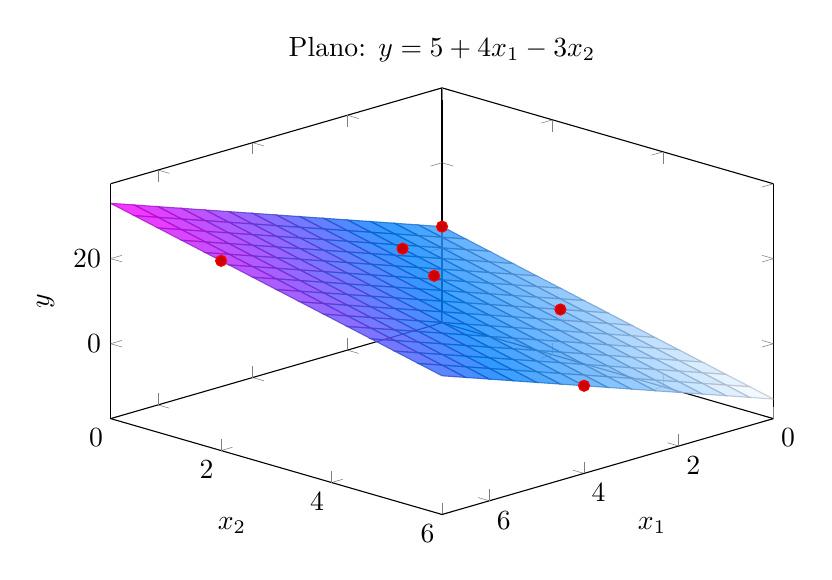
\begin{tikzpicture}
    \begin{axis}[
      view={135}{30},
      width=10cm,
      height=7cm,
      xlabel={$x_1$},
      ylabel={$x_2$},
      zlabel={$y$},
      mesh/ordering=y varies,
      domain=0:7,
      y domain=0:6,
      samples=15,
      samples y=15,
      colormap/cool,
      title={Plano: $y = 5 + 4x_1 - 3x_2$}
    ]
    % Plano ajustado
    \addplot3[surf, opacity=0.8] {5 + 4*x - 3*y};

    % Puntos originales
    \addplot3+[only marks, mark=*] coordinates {
      (0,0,5) (2,1,10) (2.5,2,9)
      (1,3,0) (4,6,3) (7,2,27)
    };
    \end{axis}
  \end{tikzpicture}
  \end{center}
\end{frame}

\end{document}